\chapter{Architektur}

\section{Die Spieleverwaltung}
\sectionauthor{\frank}

Ziel eines derartigen Frameworks ist, dieses möglichst modular \unsure{Ist das
das Ziel?} zu entwickeln. Dazu gehört auch, es zu ermöglichen, Spiele einfach
und dynamisch hinzufügen zu können. Sicher könnte man dessen benötigten Klassen
erstellen und anschließend an irgendeiner Stelle in die App hardcoden. Doch wir
wollten diesen ganzen Prozess vereinfachen, und damit flüssiger, angenehmer und
vor allem modularer gestalten. Dadurch wird auch das Ändern oder Löschen von
Spielen vereinfacht. Außerdem wird so der Weg für zukünftige Automatisierung --
wie beispielsweise Spielständen -- geebnet.

\subsection{Deklaration von Spielen}

Die Deklaration von Spielen erfolgt strukturiert in einer XML-Datei, welche
durch eine \textbf{Document Type Definition} semantisch abgesichert ist. So
wird gewährleistet, dass die Spiele im passenden Format vorliegen und so
entsprechend weiterverarbeitet werden können. Die Datei erlaubt außerdem die
Zuordnung in selbst gewählte Spiele-Kategorien, wie zum Beispiel
\emph{Kartenspiele} oder \emph{Brettspiele}.

\change{Bessere Graphik und Caption}
\begin{figure}[h]
	\centering
	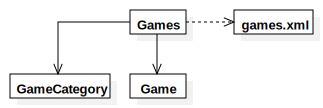
\includegraphics{resources/gamemanager/gamemanager_uml}
	\caption{Test}
	\label{fig:gm_uml}
\end{figure}
